%!TEX root = main.tex
\chapter[Evaluaci\'on]{Evaluaci\'on}
\label{sec:evaluation}

\section{Evaluation}

In this section we perform an evaluation of our introduced mutation operator \emph{prvo}. The objective of the evaluation is to analyze whether this new mutation operator indeed contributes to mutation testing, i.e., it does not lead to redundant mutants, and it can be effectively used, in terms of its associated cost, as part of mutation analysis. Our analysis ir organized around the following research questions:  
\begin{itemize}
	
	\item \textbf{RQ1} Does \emph{prvo} significantly complement traditional mutation operators?
	
	\item \textbf{RQ2} What is the added cost of using \emph{prvo} as an additional mutation operator, for mutation analysis?
	
\end{itemize}

We have already discussed the motivation for \textbf{RQ1}; a new operator would not be useful if it is redundant with respect to operators already deemed sufficient. In order to answer \textbf{RQ1}, we will perform dynamic subsumption analysis, using a benchmark of object-oriented data structure implementations, in Java. The reason for considering such a benchmark is that, in this kind of implementations, there is a substantial use of navigational expressions, including recursive datatypes, etc. Subjects will be composed of the following collections implementations: \emph{Apache's TreeList}, a tree implementation of lists; \emph{Apache's NodeCachingList}, a linked list with a node cache; \emph{AvlTree}, a classic implementation of balanced trees; \emph{BinomialHeap}, a sophisticated reference-based implementation of heaps; \emph{Queue}, a custom reference-based implementation of queues, introduced as our motivating example; and \emph{TreeSet}, a red-black tree implementation of sets. Experiments were run on desktops featuring Intel Core i7 7700HQ CPUs at 2.8GHz, 16GM of RAM, and running GNU/Linux. We report, besides subsumption results, other useful information: mutants generated, surviving mutants, and mutation score. For surviving \emph{prvo} mutants we analyzed if they were equivalent (this was manually tested), the remaining being considered non-trivial. 


In order to perform dynamic subsumption analysis, we have to provide test suites too. Moreover, for the analysis to be meaningful, we should concentrate on relatively ``good'' test sets, since with poor suites (low coverage values, for instance) we may obtain either no relationship between mutants, or spurious relations (some that only hold due to being evaluated with poor suites). Also, suites should be composed of a reasonably large set of test cases (so that one can observe subsumption relations). We will generate suites automatically, for this analysis. But in order to comply with the above restrictions, we will use a combination of two different test generation tools, Evosuite \cite{evosuite} and Randoop \cite{randoop}. Evosuite, being guided by coverage criteria, provides us with a baseline test suite with high coverage and mutation score, whereas Randoop, being random, contributes with larger test sets, that can be generated very efficiently, to complement EvoSuite's generated suites. We use EvoSuite with branch coverage and weak mutation as goals, and Randoop with its standard default configuration. Both EvoSuite and Randoop are run for 30 seconds each, and the obtained suites are combined for the analysis. Each experiment is repeated 30 times with different, randomly selected seeds. 


The analysis has to take into account \emph{prvo} as an additional operator, of course. We implemented \emph{prvo} and incorporated it into \emph{muJava} \cite{mujava}, a well-known source-code based mutation testing tool for Java. The reason is simple: \emph{muJava} performs a sophisticated parsing to implement mutations, which allowed us to incorporate \emph{prvo} relatively easily in this setting; this is in contrast with other tools for mutation testing where mutation operators are defined, typically, as expression replacement rules (\emph{prvo} cannot be implemented using such a simple strategy). The other mutation operators considered in the analysis are the \emph{method mutations} provided in \emph{muJava}, which include the sufficient mutation operators \cite{sufficient-mut-ops}, as well as various others. We refer the reader to \cite{muJavaMOPS} for details on all method-level mutations supported by \emph{muJava}, which we used in our analyses.  

Subsumption analysis results can be presented through \emph{subsumption graphs}. In these graphs, node are set of equivalent mutants (mutants that subsume one another), and an edge connects two nodes $a$ and $b$ iff mutants in $a$ subsume those in $b$. 

We also want to analyze the impact of \emph{prvo} in mutation scores. For this reason, we repeated all experiments with and without \emph{prvo} set, and compared the corresponding mutation scores obtained.

Regarding \textbf{RQ2}, the focus is on efficiency; even though \emph{prvo} (or any other operator, for that matter) may be worthwhile, its use is prohibitive if its associated cost is too high. Two factors typically govern the operator's associated cost in mutation testing: the complexity for generation, and the number of generated mutants. The former is typically disregarded, since its running time is negligible. The latter is usually considered the main driving concern for a mutation operator, since in the worst case all tests must be executed for all mutants to compute a mutation score. It is the one we concentrate on here, assessing it in terms of the generated mutants, with and without considering \emph{prvo}, for comparison. 

Due to space restrictions, we only report here a summary of the experimental results. Further information, along with a replication package, can be found in:
\begin{center}
	\texttt{https://sites.google.com/view/prvo/}
\end{center}


\subsection{Experimental Results}

Let us now discuss the results of our evaluation, focusing first on \textbf{RQ1}. Figure~\ref{subsumption-results} summarizes the results of our subsumption analysis. Results are shown per case study. Each chart includes the percentage of dominator mutants per mutation operator, using the median of all runs for the same case study. These were run, as explained earlier in this section, twice; first, without considering \emph{prvo}, only considering existing mutation operators. Results are shown in green bars. For instance, for Apache's TreeList, over 35\% of the LOI (Logical Operator Insertion) mutants were dominators, in the runs where \emph{prvo} was not considered. Obviously, there are no green bars for the PRVO column. When \emph{prvo} is taken into account, and experiments re-run, these percentages change. Percentages of dominator mutants per operator, in runs where \emph{prvo} was taken into account, are shown as red bars in the charts (again, with the median of all experiments for the same case study). For instance, for Apache's TreeList, the percentage of LOI mutants that are dominators is decreased to less than 30\% when \emph{prvo} is considered. Also, for this same case study, the percentage of dominator mutants associated with \emph{prvo} is 25\%. 

There is one last piece of information highlighted in Figure~\ref{subsumption-results}. Recall that, when building subsumption graphs to perform dynamic subsumption analysis, all mutants that dominate each other are ``collapsed'' as a single node. Thus, if such a node is ``dominator'' in the graph, all mutation operators that contributed mutants to the set are considered dominators. For the case of \emph{prvo}, we would like to know which dominator nodes are \emph{only} composed of \emph{prvo} mutants. We show that information in the charts with a blue bar. For instance, for Apache's TreeList, over 20\% of the dominator mutants in the runs where \emph{prvo} was considered were ``pure'' \emph{prvo}, i.e., they were not accompanied as subsumers by mutants other than \emph{prvo} ones. 

Let us now analyze these results. The most important observation is that in almost all case studies (with the exception of Apache's NodeCachingList), \emph{prvo} is among the top operators in terms of dominance. Indeed, \emph{prvo} is in general one of the top three dominator operators, accompanying typical ``sufficient'' mutators, such as ROR (Relational Operator Replacement, LOI, or the family of Arithmetic Operator Insertion operators (AOIS, AOIU, AOIB, \dots). Also, it is important to remark that, in the presence of \emph{prvo}, the dominance of other operators is in general decreased, as their dominance over some nodes is ``transferred'' towards \emph{prvo}. More precisely, \emph{prvo} ``dominates'' some ``root'' mutants, i.e., mutants that in the absence of \emph{prvo} are dominators.    

Clearly, our experimental results support a positive answer to \textbf{RQ1}, i.e., \emph{prvo} does in fact significantly complement traditional mutation operators; it generally produces a large set of mutants not dominated by existing operators, and exhibits a high number of dominant mutants, that may even allow us, at least in the context of our experiments, to consider \emph{prvo} a sufficient operator (along with the traditional sufficient ones). 

\begin{figure}[t]
	\begin{center}
		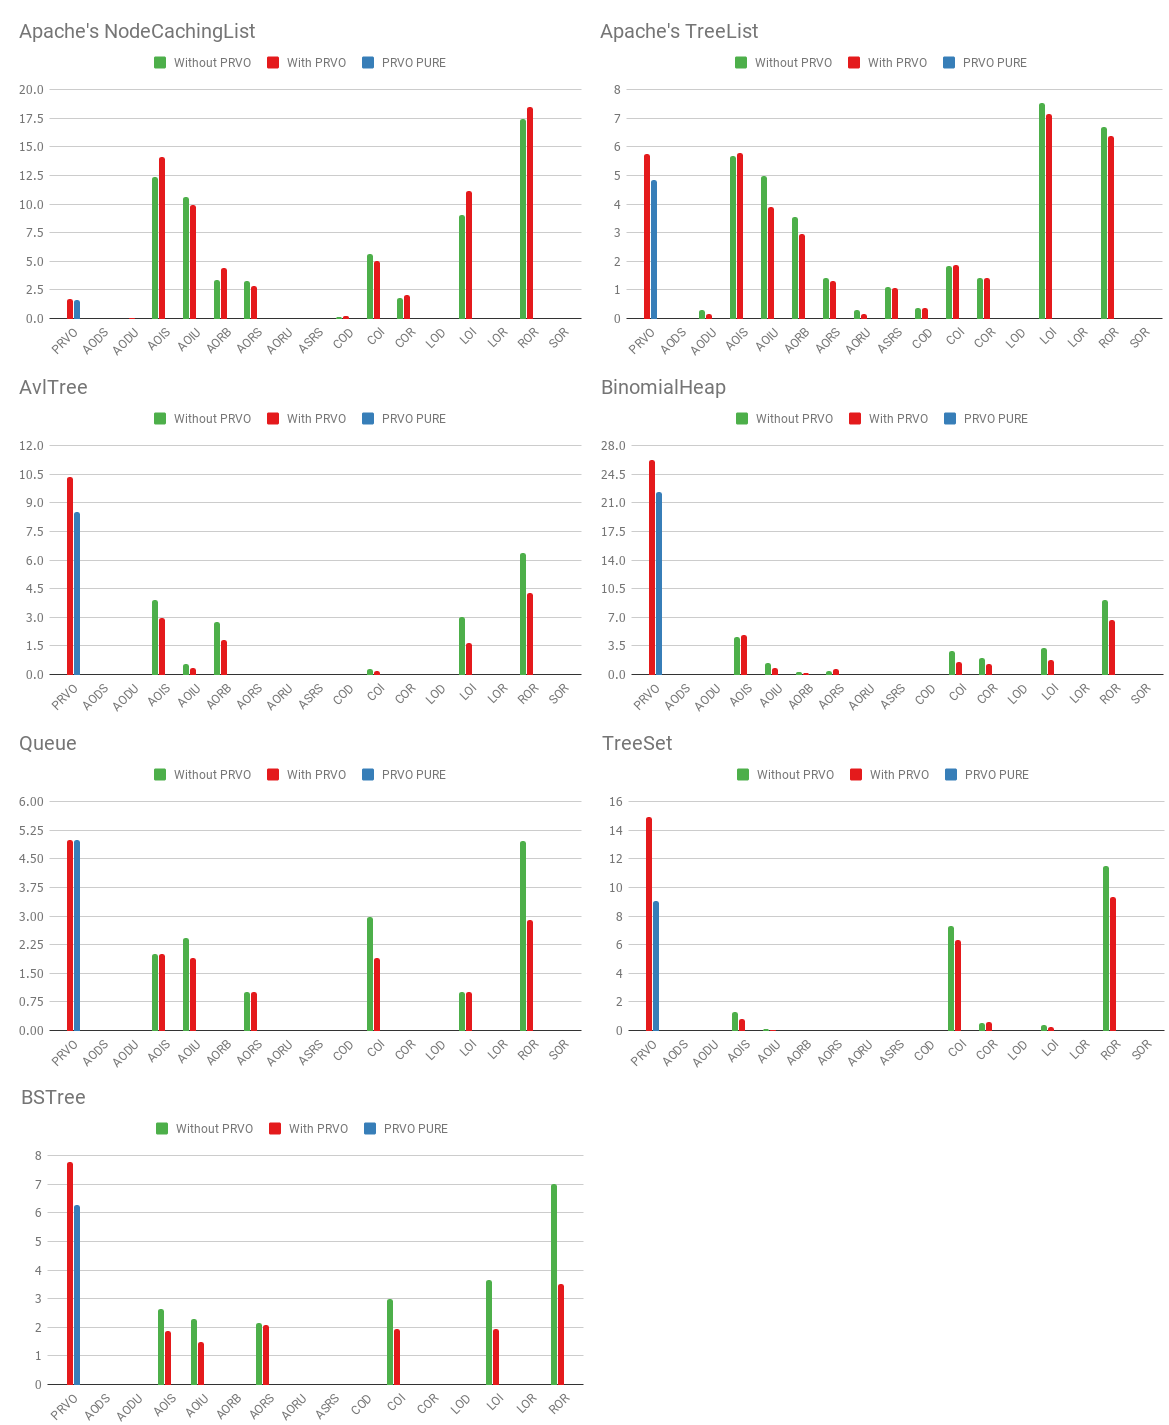
\includegraphics[width=12cm]{figures/Tables.png}
	\end{center}
	\caption{Summary of dynamic subsumption analysis}
	\label{subsumption-results}
\end{figure}

Now let us turn our attention to \textbf{RQ2}. Figure~\ref{mutants-results} summarizes the results for mutants generation, comparing the number of mutants obtained when \emph{prvo} is disabled (green bars) with those for the cases in which \emph{prvo} is enabled (blue bars). We also report in this summary the number of equivalent \emph{prvo} mutants (i.e., mutants that are semantically equivalent to the original program, and thus cannot be killed no matter which tests we consider) produced for each case study.

For the majority of the case studies, the number of mutants that \emph{prvo} generates is a small ``overhead'' over the set of mutants generated when \emph{prvo} is disregarded. TreeSet and BinomialHeap are two exceptions, where \emph{prvo} alone generates roughly the same number of mutants as all the other operators together. The reason is that these case studies feature methods with a high number of navigational expressions in conditions and other comparisons, of the kind \texttt{expr == null}. These expressions admit a single ROR mutation (replacing equals by not equals), whereas \emph{prvo} produces many more mutations from the same mutation point. Notice however that in these two case studies, \emph{prvo} is a clear dominator (see Figure~\ref{subsumption-results}); in particular, it is noticeable how the dominance of other operators is significantly diminished when \emph{prvo} is taken into account. Our preliminary answer to \textbf{RQ2} is then that the added cost associated with \emph{prvo} is in general low, although there are cases where the number of \emph{prvo} mutations may explode. These cases show, in our experiment, a greater dominance of \emph{prvo} over other mutations, suggesting that there is margin for optimization via test/mutant prioritization in these cases. Still, these results call for refinements to \emph{prvo}, that may lead to a consistently low overhead in mutation analysis, with respect to traditional mutations.

Regarding equivalent mutants, the results are interesting too. A very low number of mutants were equivalent to the original program. Notice that this is an important number. When an operator produces many equivalent mutants, the corresponding mutation scores are artificially (and misleadingly) reduced, since having mutants that cannot be killed will make scores to tend towards lower number. Having small numbers of such mutants is then clearly a good sign.     



\begin{figure}[t]
	\begin{center}
		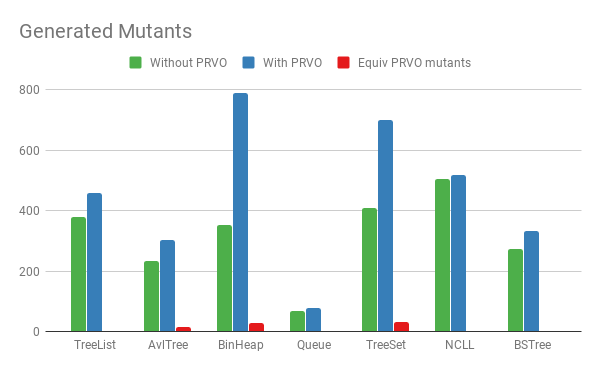
\includegraphics[width=9cm]{figures/Generated_Mutants.png}
	\end{center}
	\caption{Summary of mutants generated.}
	\label{mutants-results}
\end{figure}


\subsection{Threats to validity}

Our experimental evaluation is limited to relatively small, stateful Java implementations of collections. The reasons for selecting these implementations as our benchmark have been partially described before, and essentially have to do with these projects being good representatives of object-oriented implementations with sophisticated uses of navigations (e.g., over recursive datatypes, with multiple (non-aliased) references to objects of the same type, etc. Another reason for limiting ourselves to these case studies has to do with the high cost of mutation analysis. Especially in our context, where due to the inherent characteristics of these investigations we had to perform numerous mutation analyses, selecting larger projects would imply a cost, in particular in computing subsumption graphs, that would make our evaluation infeasible. 

Our analysis is also tied to a very specific way of generating tests, that we have described earlier in this paper. It is also motivated by the kind of test suites that would be relevant for subsumption analysis. Our results may however be biased by the specific timeout selected for test generation. We have therefore run our experiments with different timeouts, leading to test suites of different sizes, and of course different analysis results. Results are however consistent with those presented in the paper. Further details regarding the various runs with varying timeouts, as well as further experimental information, can be found in \texttt{https://sites.google.com/view/prvo/}. 

Most of our experimental evaluation is rather objective, e.g., the notion of subsumption, and are checked by our implementation. We made our best effort to check soundness of our results, but of course our implementation may contain defects affecting our results. Program equivalence, required to analyze equivalent mutants, is an undecidable problem. So our analysis in this respect was manual. Different contributors to this paper checked equivalence independently, to reduce overseen errors. Still, this analysis is fortunately only limited to a small percentage of mutants, those that were not killed by any test (the others, having been killed, are clearly non-equivalent). We believe that the errors we may have committed regarding mutant equivalence would not significantly affect our conclusions. 

Our analysis is also limited to an arbitrary set of mutation operators. Other operators, for instance class-level ones \cite{bibliography.mutation.class-level-ops}, may have been considered. These class-level operators are definitely related to our work in the sense that they apply to object-oriented programs, but they inspect orthogonal issues, such as visibility (changing the visibility of methods and fields in a class). We decided to concentrate on what are considered traditional mutation operators, in the context of mutation testing, and we believe we have taken into account the most significant existing mutations, based on what is available in mutation testing tools. 

Let us once again remark that operator subsumption is not the same as mutants subsumption. We have assessed the latter, as a way of indirectly measuring the former (the one we are actually interested in), for the reasons stated earlier in the paper (dealing directly with operator subsumption is infeasible). 

